\section[Useful Properties of Linear Algebra]{Useful Properties of Linear Algebra}

\begin{frame}{Useful Properties of Linear Algebra}
	In this section, we will exploit several highly useful properties of linear algebra to:
	\begin{itemize}
		\item \textbf{determine} the principal components, 
		\item \textbf{interpret} the results from both a \textit{geometric} and a \textit{statistical} perspective,
		\item \textbf{simplify} the statistical learning problem via a \textit{partial} change of basis for the input features $X$.
	\end{itemize}
\end{frame}

\subsection[Covariance Matrix]{Covariance Matrix}

\begin{frame}{Characteristics of the Covariance Matrix}
	\begin{itemize}
		\item The covariance matrix computed on the columns of $X$, denoted by $\Sigma \in \mathcal{M}_{p,p}(\R)$, is a \textbf{square} and \textbf{symmetric} matrix by design, thanks to the symmetry of the covariance operator.
		\pause
		\item It is also \textbf{positive semi-definite}. For any vector $v \in \mathcal{M}_{p,1}(\R)$, it can be shown that $v^T \Sigma v \ge 0$.
		\pause
		\item Because it is symmetric, its eigenvectors $u$ are mutually \textbf{orthogonal}, and its eigenvalues are \textbf{real} numbers.
		\pause
		\item Furthermore, because it is positive semi-definite, its eigenvalues $\lambda$ are necessarily \textbf{non-negative} ($\lambda \ge 0$).
	\end{itemize}
\end{frame}

\begin{frame}{Spectral Decomposition of the Covariance Matrix}
	The spectral decomposition (or eigen-decomposition) of the covariance matrix is given by:
	\begin{equation}
		\Sigma = U \Lambda U^T
		\nonumber
	\end{equation}
	Where $U \in \mathcal{M}_{p,p}(\R)$ is an orthogonal matrix ($U^T U = I_p$, meaning $U^T = U^{-1}$) whose columns are the eigenvectors:
	\begin{equation}
		U = \begin{pmatrix}
			\vert & \vert & \cdots & \vert \\
			u_1   & u_2   & \cdots & u_p   \\
			\vert & \vert & \cdots & \vert
		\end{pmatrix}
		\nonumber
	\end{equation}
	And $\Lambda \in \mathcal{M}_{p,p}(\R)$ is a diagonal matrix containing the eigenvalues:
	\begin{equation}
		\Lambda = \begin{pmatrix}
			\lambda_1 & 0 & \cdots & 0 \\
			0 & \lambda_2 & \cdots & 0 \\
			\vdots & \vdots & \vdots & \vdots \\
			0 & 0 & \cdots & \lambda_p
		\end{pmatrix} \quad \text{with} \quad \lambda_1 \ge \lambda_2 \ge \dots \ge \lambda_p
		\nonumber
	\end{equation}
\end{frame}

\begin{frame}{Graphical Representation}
	\begin{columns}
		\begin{column}{0.5\textwidth}
			\begin{figure}
				\centering
				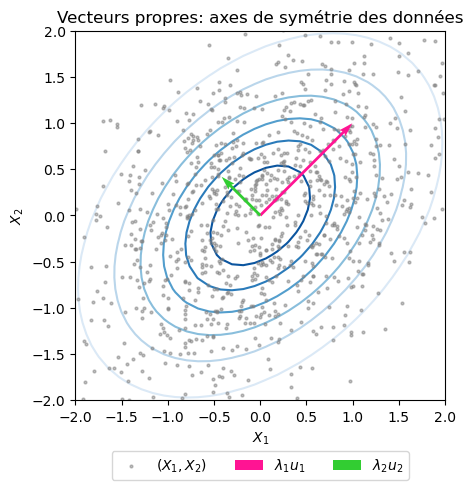
\includegraphics[height=1.0\linewidth]{Images/axes_de_symétrie}
				\label{fig:axes_de_symetrie}
			\end{figure}			
		\end{column}
		\begin{column}{0.5\textwidth}
			The accompanying figure illustrates the idealized contour lines (iso-probabilities) representative of a covariance matrix in $\R^2$. The eigenvector of the first principal component aligns with the major axis, whereas the eigenvector of the second principal component aligns with the minor axis. The eigenvalues represent the lengths of the axes of these ellipses.
		\end{column}
	\end{columns}
\end{frame}

\begin{frame}{Change of Basis}
	The matrix $U$ acts as the change-of-basis matrix from the original basis $\mathcal{B}$ (associated with the feature space $\mathcal{X}$) to a new basis $\mathcal{B}^{'}$ where the covariance matrix becomes diagonal. The matrix $U^T$ represents the inverse transformation from $\mathcal{B}^{'}$ back to $\mathcal{B}$:
	\begin{equation}
		\Lambda = U^T \Sigma U
		\nonumber
	\end{equation}
	In this new basis $\mathcal{B}^{'}$, the features no longer share any linear interdependence; they are completely uncorrelated.
\end{frame}

\begin{frame}{Change of Basis}
	The change of basis from $\mathcal{B}$ to $\mathcal{B}^{'}$ for the observed input feature matrix $X$ is written as:
	\begin{equation}
		Z = X U
		\nonumber
	\end{equation}
	The score matrix $Z \in \mathcal{M}_{n,p}(\R)$ now incorporates all $p$ principal components.
\end{frame}

\begin{frame}{Change of Basis}
	Below is an example of a full change of basis utilizing all eigenvectors within a two-dimensional feature space $\R^2$:
	\begin{figure}
		\centering
		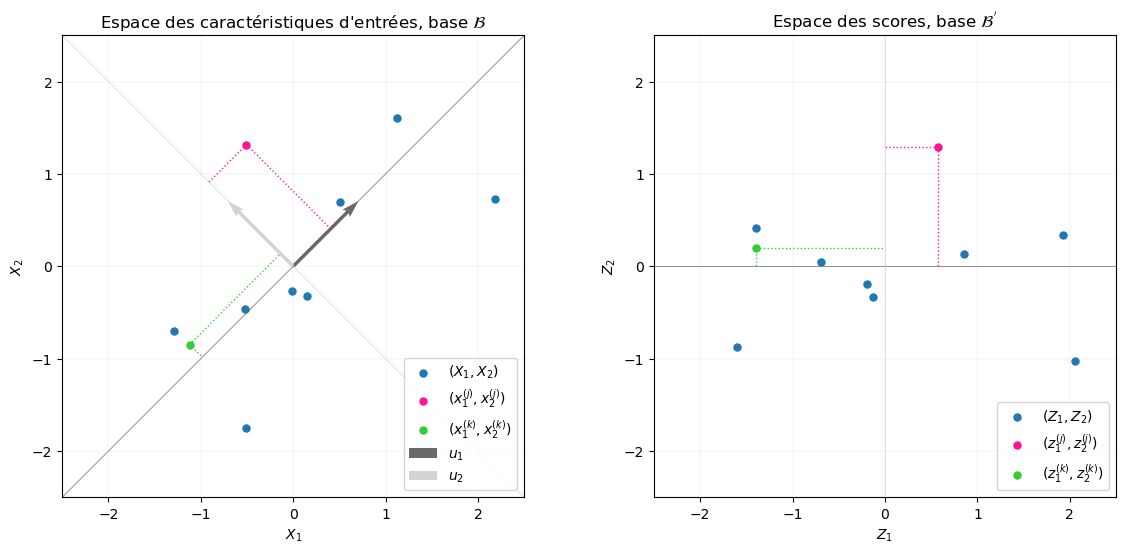
\includegraphics[width=0.95\linewidth]{Images/changement_de_base}
		\label{fig:changement_de_base}
	\end{figure}
\end{frame}

\subsection[Finding Eigenvalues and Eigenvectors]{Finding Eigenvalues and Eigenvectors}

\begin{frame}{Definition of Eigenvalues and Eigenvectors}
	A symmetric matrix $\Sigma \in \mathcal{M}_{p,p}(\R)$ admits a scalar $\lambda \in \R$ as an eigenvalue and a non-zero vector $u \in \mathcal{M}_{p,1}(\R)$ as its associated eigenvector if and only if:
	\begin{equation}
		\Sigma u = \lambda u
		\nonumber
	\end{equation}
	Thus, the transformation of $u$ by $\Sigma$ results in a vector collinear to $u$. \\
	\pause
	\vspace{0.5cm}
	An equivalent expression is:
	\begin{equation}
		\Sigma u - \lambda u = 0 \iff \left(\Sigma - \lambda I_p\right) u = 0
		\nonumber
	\end{equation}
	Since we are looking for a non-zero vector $u$, and because the zero vector is a trivial solution to this linear system, the matrix $\left(\Sigma - \lambda I_p\right)$ must necessarily be \textbf{singular}.
\end{frame}

\begin{frame}{Characteristic Equation of Matrix $\Sigma$}
	If the matrix $\left(\Sigma - \lambda I_p\right)$ is singular, its determinant must be zero:
	\begin{equation}
		\det \left(\Sigma - \lambda I_p\right) = 0
		\nonumber
	\end{equation}
	The solutions to this \textbf{characteristic equation}, which is nonlinear in $\lambda$, provide the eigenvalues of the matrix $\Sigma$.
\end{frame}

\begin{frame}{Graphical Representation}
	In a two-dimensional space $\R^2$, the figures below illustrate the linear transformation (endomorphism) operated on the space by a symmetric matrix. Points located on the lines representing the principal components remain on those identical lines, either moving closer to the origin (eigenvalue smaller than 1) or moving farther away (eigenvalue greater than 1):
	\begin{columns}
		\begin{column}{0.5\textwidth}
			\begin{figure}
				\centering
				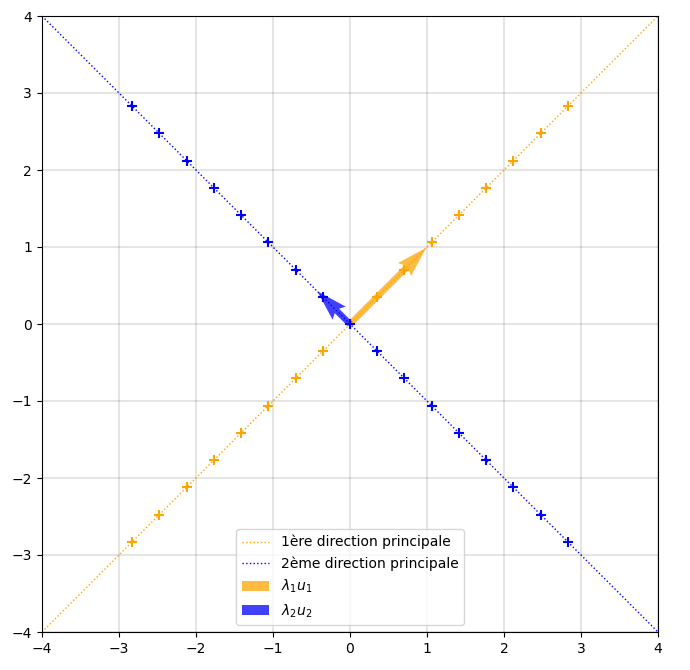
\includegraphics[height=0.85\linewidth]{Images/vecteur_valeur_propre_1}
				\label{fig:vecteur_valeur_propre_1}
			\end{figure}			
		\end{column}
		\begin{column}{0.5\textwidth}
			\begin{figure}
				\centering
				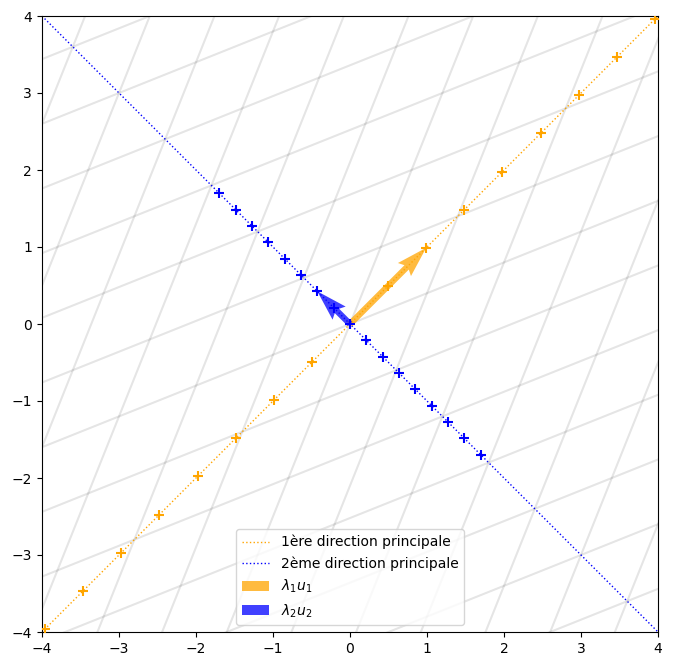
\includegraphics[height=0.85\linewidth]{Images/vecteur_valeur_propre_2}
				\label{fig:vecteur_valeur_propre_2}
			\end{figure}			
		\end{column}
	\end{columns}
\end{frame}

\subsection[Trace of the Covariance Matrix]{Trace of the Covariance Matrix}

\begin{frame}{Trace of the Covariance Matrix}
	The trace of a covariance matrix is defined as the sum of its diagonal elements. Therefore:
	\begin{equation}
		\operatorname{Tr}(\Sigma) = \displaystyle \sum_{j=1}^p \Varhat{X_{\bigdot j}}
		\nonumber
	\end{equation}
	\pause
	Hence, the trace \textit{captures} the \textbf{total variance} of all the individual input features. Since the trace of a matrix is \textbf{invariant under a change of basis}, we can write:
	\begin{equation}
		\operatorname{Tr}(\Sigma) = \displaystyle \sum_{j=1}^p \Varhat{X_{\bigdot j}} = \sum_{j=1}^p \lambda_j
		\nonumber
	\end{equation}
	An interpretation of this identity is that the diagonal matrix $\Lambda$ has \textbf{completely redistributed} the variance of the original features across the eigenvalues, while eliminating all feature interdependencies.
\end{frame}

\begin{frame}{Scree Plots and Eigenvalue Ratios}
	A consequence of this property is that each individual eigenvalue $\lambda_k$ represents a distinct fraction of the total variance of the columns of $X$:
	\begin{equation}
		\text{Ratio} = \frac{\lambda_k}{\sum_{j=1}^p \lambda_j}
		\nonumber 
	\end{equation}
	\pause
	This property serves as the cornerstone of Principal Component Analysis:
	\begin{block}{Simplification Principle of PCA}
		The simplification relies on selecting the top $k$ eigenvalues that capture a \textit{sufficient} fraction of the total variance required for the statistical learning problem.
	\end{block}
\end{frame}

\begin{frame}{Example of Eigenvalue Scree Plots}
	\begin{columns}
		\begin{column}{0.5\textwidth}
			\begin{figure}
				\centering
				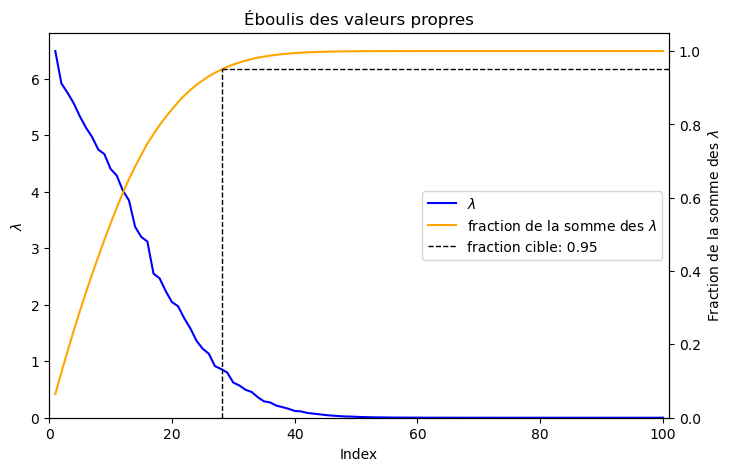
\includegraphics[width=1.0\linewidth]{Images/eboulis}
				\label{fig:eboulis}
			\end{figure}			
		\end{column}
		\begin{column}{0.5\textwidth}
			In the adjacent plot:
			\begin{itemize}
				\item We observe how the eigenvalues decrease sharply from the first principal component to the last.
				\item The cumulative sum curve of the $\lambda$ ratios (the cumulative explained variance ratio) shows that selecting the first 30 principal components preserves 95\% of the total variance.
			\end{itemize}
		\end{column}
	\end{columns}	
\end{frame}

\subsection[Dimensionality Reduction]{Dimensionality Reduction}

\begin{frame}{Simplification via Partial Score Computation}
	The problem simplification process consists of selecting the top $k \in \mathbb{N}$ largest eigenvalues $\lambda_1, \lambda_2, \dots, \lambda_k$ with $k < p$, alongside their associated eigenvectors $u_1, u_2, \dots, u_k$, to compute a partial score matrix $Z^* \in \mathcal{M}_{n,k}(\R)$:
	\begin{equation}
		Z^* = X U^*
		\nonumber
	\end{equation}
	Where $U^* \in \mathcal{M}_{p,k}(\R)$ is defined as:
	\begin{equation}
		U^* = \begin{pmatrix}
			\vert & \vert & \cdots & \vert \\
			u_1   & u_2   & \cdots & u_k   \\
			\vert & \vert & \cdots & \vert
		\end{pmatrix}
		\nonumber
	\end{equation}
	This partial score matrix preserves a fraction of the original column variance of $X$ given by the ratio:
	\begin{equation}
		\text{Ratio} = \frac{\sum_{j=1}^k \lambda_j}{\sum_{j=1}^p \lambda_j}
		\nonumber
	\end{equation}
\end{frame}

\begin{frame}{Reconstruction via Projection}
	Using partial projection, we can reconstruct an approximation matrix $\hat{X} \in \mathcal{M}_{n,p}(\R)$ from $Z^*$:
	\begin{equation}
		\begin{aligned}
			\hat{X} &= Z^* U^{*T} \\
			&= X U^* U^{*T}
		\end{aligned}
		\nonumber
	\end{equation}
	\pause
	This reconstruction of $X$ is inherently imperfect since a portion of the variance was discarded during the process. The error matrix is defined as:
	\begin{equation}
		\text{Error} = X - \hat{X}
		\nonumber
	\end{equation}
\end{frame}

\begin{frame}{Reconstruction via Projection}
	In the special case where we retain \textbf{all} eigenvalues, we obtain a perfect reconstruction with zero error. Indeed, since the full matrix $U$ is orthogonal:
	\begin{equation}
		\begin{aligned}
			\hat{X} &= X U U^T \\
			&= X I_p \\
			&= X
		\end{aligned}
		\nonumber
	\end{equation}
\end{frame}

\subsection[Summary]{Summary}

\begin{frame}{Methodology of Principal Component Analysis}
	\begin{enumerate}
		\item Compute the covariance matrix $\Sigma \in \mathcal{M}_{p,p}(\R)$ from the $p$ columns of the $n$ standardized observations $X \in \mathcal{M}_{n,p}(\R)$.
		\pause
		\item Determine the eigenvectors $u_1, u_2, \dots, u_p$ and their associated eigenvalues $\lambda_1, \lambda_2, \dots, \lambda_p$ ordered such that $\lambda_1 \ge \lambda_2 \ge \dots \ge \lambda_p$. Note that $u_j \in \mathcal{M}_{p,1}(\R)$ and $\lambda_j \in \R^+$ for all $j=1, 2, \dots, p$.
		\pause
		\item Select the top $k \le p, k \in \mathbb{N}$ largest eigenvalues based on the targeted fraction of variance to preserve, and form the partial projection matrix $U^* \in \mathcal{M}_{p,k}(\R)$ using the $k$ corresponding eigenvectors.
		\pause
		\item The proportion of preserved variance is given by: $\text{Ratio} = \left(\sum_{j=1}^k \lambda_j\right) / \left(\sum_{j=1}^p \lambda_j\right)$.
		\pause
		\item \textbf{Compress} the observed data $X$ into partial scores $Z^* = X U^*$, where $Z^* \in \mathcal{M}_{n,k}(\R)$.
		\pause
		\item \textbf{Decompress} the scores back into feature space to obtain $\hat{X}$: $\hat{X} = Z^* U^{*T}$.
		\pause
		\item Quantify the distortion or information loss introduced by data compression using the error matrix: $\text{Error} = X - \hat{X}$.
	\end{enumerate}
\end{frame}